\tikzstyle{input_neuron}=[circle,draw=red!50,fill=red!10,thick,minimum size=6mm]
\tikzstyle{hidden_neuron}=[circle,draw=blue!50,fill=cyan!10,thick,minimum size=6mm]
\tikzstyle{output_neuron}=[circle,draw=green!50,fill=green!10,thick,minimum size=6mm]
\tikzstyle{input}=[circle,draw=black!50,fill=black!20,thick,minimum size=6mm]
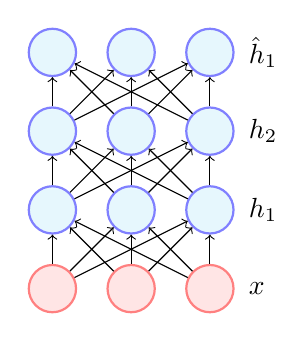
\begin{tikzpicture}	
	
	\node [input_neuron] (neuron11) at (7,2.5){}  ;
	\node [input_neuron] (neuron12) at (8,2.5){}  ;
	\node [input_neuron] (neuron13) at (9,2.5){}  ;
	\node [hidden_neuron] (neuron21) at (7,3.5){}  ;
	\node [hidden_neuron] (neuron22) at (8,3.5){}  ;
	\node [hidden_neuron] (neuron23) at (9,3.5){}  ;
	\node [hidden_neuron] (neuron31) at (7,4.5){}  ;
	\node [hidden_neuron] (neuron32) at (8,4.5){}  ;
	\node [hidden_neuron] (neuron33) at (9,4.5){}  ;
	\node [hidden_neuron] (neuron41) at (7,5.5){}  ;
	\node [hidden_neuron] (neuron42) at (8,5.5){}  ;
	\node [hidden_neuron] (neuron43) at (9,5.5){}  ;
	
	%\draw[red!100,thick,solid] (6.5,2) rectangle (9.5,4);
	\node[text width=0.01cm] at (9.5,5.5) {$\hat{h}_1$};
	\node[text width=0.01cm] at (9.5,4.5) {$h_{2}$};
	\node[text width=0.01cm] at (9.5,3.5) {$h_{1}$};
	\node[text width=0.01cm] at (9.5,2.5) {$x$};
	
	\draw [->] (neuron11) -- (neuron21);
	\draw [->] (neuron11) -- (neuron22);
	\draw [->] (neuron11) -- (neuron23);
	\draw [->] (neuron12) -- (neuron21);
	\draw [->] (neuron12) -- (neuron22);
	\draw [->] (neuron12) -- (neuron23);
	\draw [->] (neuron13) -- (neuron21);
	\draw [->] (neuron13) -- (neuron22);
	\draw [->] (neuron13) -- (neuron23);
	
	\draw [->] (neuron21) -- (neuron31);
	\draw [->] (neuron21) -- (neuron32);
	\draw [->] (neuron21) -- (neuron33);
	\draw [->] (neuron22) -- (neuron31);
	\draw [->] (neuron22) -- (neuron32);
	\draw [->] (neuron22) -- (neuron33);
	\draw [->] (neuron23) -- (neuron31);
	\draw [->] (neuron23) -- (neuron32);
	\draw [->] (neuron23) -- (neuron33);
	
	\draw [->] (neuron31) -- (neuron41);
	\draw [->] (neuron31) -- (neuron42);
	\draw [->] (neuron31) -- (neuron43);
	\draw [->] (neuron32) -- (neuron41);
	\draw [->] (neuron32) -- (neuron42);
	\draw [->] (neuron32) -- (neuron43);
	\draw [->] (neuron33) -- (neuron41);
	\draw [->] (neuron33) -- (neuron42);
	\draw [->] (neuron33) -- (neuron43);
	
\end{tikzpicture}